%
% 23-eudklidisch.tex -- Euklidische Ringe
%
% (c) 2026 Prof Dr Andreas Müller
%
\subsection{Euklidische Ringe
\label{buch:ratint:euklid:subsection:ringe}}
Der euklidische Algorithmus benötigt erst mal, dass es keine
pathologischen Faktoren gibt, die ein Produkt auslöschen können.
Solche pathologischen Fälle führen dazu, dass es nicht sinnvoll ist
von einer eindeutigen Faktorisierung zu sprechen.
Pathologische Faktoren heissen Nullteiler im Sinne der folgenden
Definition.

\begin{definition}[Nullteiler, Integritätsbereich]
Nullteiler \emph{Nullteiler} in einem Ring $R$ sind Zahlen
$a,b\in R^*=R\setminus\{0\}$ mit $ab=0$.
Ein Ring $R$ ohne Nullteiler heisst \emph{nullteilerfrei} oder ein
\emph{Integritätsbereich}.
\index{Nullteiler}%
\index{nullteilerfrei}%
\index{Integritatsbereich@Integritätsbereich}%
\end{definition}

Die ganzen Zahlen und die Menge der Polynome bilden Integritätsbereiche.

Der euklidische Algorithmus für ganze Zahlen verwendet, dass der Rest
bei der ganzzahligen Division kleiner als der Divisor ist.
Polynome kann man nicht vergleichen.
Der euklidische Algorithmus für Polynome braucht aber, dass der Grad
des Restes kleiner wird als der Grad des Divisors.
Der Algorithmus ist also auf eine allgemeinere Situation übertragbar,
wenn ein Eigenschaft ähnlich dem Grad gefunden werden kann, die bei
der Division kleiner wird.

\begin{definition}[Euklidischer Ring]
\label{buch:ratint:euklid:def:euklidischerring}
Ein nullteilerfreier Ring  $R$ heisst ein \emph{euklidischer Ring},
\index{euklidischer Ring}%
\index{Ring!euklidisch}%
wenn es eine Funktion $d\colon R^*\to\mathbb{Z}$
\begin{enumerate}
\item $d(r) \ge 0$ für alle $r\in R^*$.
\item $d(r)\le d(rs)$ für alle $r,s\in R^*$.
\item Sind $a,b\in R^*$, dann gibt es $q,r$ mit $a=qb+r$ mit $r=0$ oder
$d(r)<d(b)$.
\end{enumerate}
Die Funktion $d$ heisst auch die \emph{Gradfunktion} des euklidischen
Rings.
\index{Gradfunktion}%
Die letzte Eigenschaft kann etwas vereinfacht werden, wenn man
$d(0)=-\infty$ definiert.
\end{definition}

Für die ganzen Zahlen ist die $d\colon\mathbb{Z}^*\to\mathbb{Z}: a\to a$
die Funktion, die die ganzen Zahlen zu einem euklidischen Ring macht.
Für Polynome mit Koeffizienten in einem Körper ist es der Grad
$\deg\colon K[X] \to \mathbb{Z} : p(X) \mapsto \deg p$.

Ein weiteres interessantes Beispiel für einen euklidischen Ring ist
der Ring der ganzen gaussschen Zahlen.

\begin{beispiel}
Wir betrachten die Menge
\[
\mathbb{Z}[i]
=
\{a+bi\mid a,b\in\mathbb{Z}\}\subset\mathbb{C}.
\]
Sie heisst der \emph{Ring der ganzen gaussschen Zahlen}.
\index{ganze gausssche Zahlen}%
\index{gausssche Zahlen}%
Als Teilmenge des Körpers der komplexen Zahlen ist $\mathbb{Z}[i]$
sicher ein nullteilerfreier Ring.
Als Gradfunktion kann das Betragsquadrat 
\[
d
\colon
\mathbb{Z}[i] \to \mathbb{Z}
:
(a+bi) \mapsto a^2+b^2
\]
verwendet werden.
Es müssen die drei Eigenschaften der 
Definition~\ref{buch:ratint:euklid:def:euklidischerring}
verifizieren.
\begin{enumerate}
\item
Für $a+bi\ne 0$ ist $d(a+bi)=a^2+b^2>0$.
\item
Für das Produkt gilt für $(a+bi)\ne 0$ ist $d(a+bi)\ge 1$
\[
d\bigl(
(a+bi)(c+di)
\bigr)
=
(a^2+b^2)(c^2+d^2)
=
d(a+bi)d(c+di)
\ge
d(c+di)
\]
für all $c+di\in \mathbb{Z}[i]$.
\item
Diese Eigenschaft wird am einfachsten auf die folgende geometrische
Weise verständlich (Abbildung~\ref{buch:ratint:euklid:fig:ggz}).
%
% fig-ggz.tex -- eukldische Eigenschaft für ganze gaussche Zahlen
%
% (c) 2026 Prof Dr Andreas Müller
%
\begin{figure}
\centering
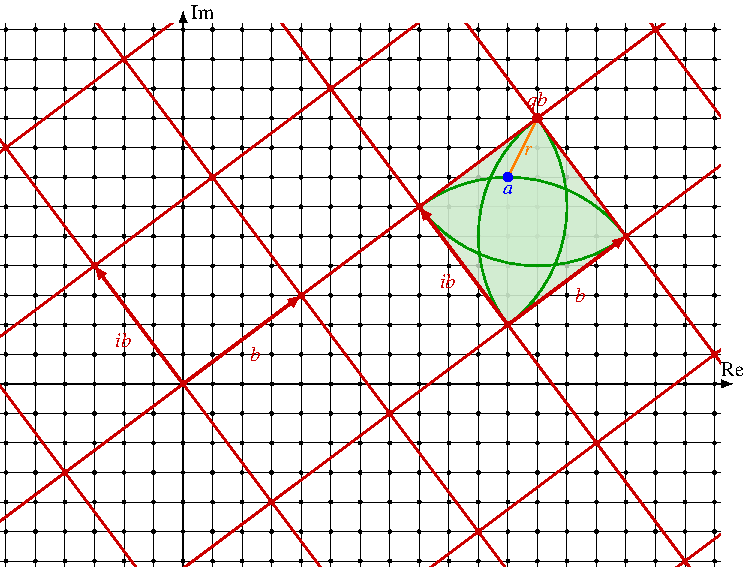
\includegraphics{chapters/060-ratint/images/ggz.pdf}
\caption{Euklidische Eigenschaft des Rings der ganzen gaussschen Zahlen.
Die Vielfachen $\mathbb{Z}[i]b= \{xb+y ib\mid x,y\in\mathbb{Z}\}$
bilden ein quadratisches Gitter ({\color{darkred}rot}). 
Die Zahl $a$ ({\color{blue}blau}) muss in einem der Gitterquadrate
({\color{darkgreen}grün}) liegen, die Seitenkanten $b$ und $ib$ haben.
Da die Kreise mit Radius $|b|$ um die Ecken das ganze Quadrat überdecken,
gibt es eine Ecke, die näher an $a$ ist als $|b|$.
Mit dem $q=x+iy$ dieser Ecke folgt $r=a-qb$ und $|r|<|b|$
bzw.~$d(r) = |r|^2 < |b|^2=d(b)$.
\label{buch:ratint:euklid:fig:ggz}}
\end{figure}
%
Die Menge 
\[
b\mathbb{Z}[i]
=
\{ zb\mid z \in \mathbb{Z}[i] \}
=
\{ xb + iyb \mid x,y\in \mathbb{Z}
\}
\]
bildet ein Gitter in der komplexen Zahlenebene.
Da $b$ und $ib$ senkrecht aufeinander stehende Vektoren sind, 
handelt es sich um ein quadratisches Gitter.
Der Punkt $a$ muss in einem der Gitterquadrate liegen.
Jede Ecke dieses Quadrats wird durch ein $q\in\mathbb{Z}[i]$
beschrieben und kommt als das $q$ in der Eigenschaft~3 eines eukldischen
Rings in Frage.
Die zusätzliche Forderung $d(r)<d(b)$ bedeutet, dass der Punkt $a$
näher als die Kantenlänge des Quadrates bei der ausgewählten Ecke
sein muss.
Da die offenen Kreisscheiben mit Radius $|b|$ die Quadratfläche 
vollständig überdecken, muss es mindestens ein $q\in\mathbb{Z}[i]$
(eine Ecke) geben,
so dass $a-qb=r$ die Bedingung $d(r) < d(b)$ ($|r|<|b|$) erfüllt ist.
\end{enumerate}
Dies zeigt, dass die ganzen gaussschen Zahlen einen euklidischen
Ring bilden.
Es ist daher sinnvoll, vom grössten gemeinsamen Teiler ganzer
gaussscher Zahlen zu sprechen und es ist möglich, diese mit dem
euklidischen Algorithmus zu finden.
\end{beispiel}

Die ganzen gaussschen Zahlen können zum Beispiel dazu verwendet
werden, dann folgenden fermatschen Zweiquadratesatz zu beweisen
\cite[Satz 10.4]{buch:luneburg}.

\begin{satz}[Fermat]
\index{Fermat, Pierre de}%
\index{Satz!von Fermat}%
Ist $p$ eine Primzahl mit $p\equiv 1\mod 4$, dann gibt es ganze
Zahlen $a,b\in\mathbb{Z}$ mit $p=a^2+b^2$.
\end{satz}



